\documentclass[dvipsnames]{beamer}

\usepackage[utf8]{inputenc}
\usepackage[brazil]{babel}
\usepackage{amsmath,amssymb,amsfonts,amsthm}
\usepackage{color}
%\usepackage{dingbat}
\usepackage{graphics}
\usepackage{hyperref}
%\usepackage[dvipsnames]{xcolor}
\usepackage{tikz}

\DeclareMathOperator*{\argmax}{arg\,max}

\usetikzlibrary{positioning,shapes,arrows}

\usetheme{Copenhagen}
\setbeamertemplate{navigation symbols}{}

\title[Redes soma-produto e sua relação com redes bayesianas]{\LARGE Redes soma-produto\\e sua relação com redes bayesianas}
\author[Tiago Madeira {\tt <madeira@ime.usp.br>}]{
  {\Large Tiago Madeira}\\
  {\footnotesize \tt <madeira@ime.usp.br>}}
\institute[PCS5708]{{\footnotesize PCS5708 -- Técnicas de Raciocínio Probabilístico em Inteligência Artificial}\\
  \ \\
  Prof. Paulo Sergio Cugnasca\\
  Escola Politécnica -- Universidade de São Paulo}
\date{Maio de 2018}

\begin{document}
  \frame{\titlepage}

  \begin{frame}
    \frametitle{Roteiro}

    \tableofcontents
  \end{frame}

  \section{Introdução}

  \subsection{Motivação}

  \begin{frame}
    \frametitle{Motivação (1/2)}

    \textbf{Redes soma-produto} (\emph{Sum-Product Network = SPN})\footnote{\scriptsize POON, H. DOMINGOS, P. Sum-Product Networks: A New Deep Architecture (2011). \emph{Uncertainty in Artificial Intelligence (UAI 2011)}} são modelos profundos tratáveis para inferência probabilística.

    % XXX: Diferente de redes bayesianas e redes de Markov, permitem computar inferência exata em tempo linear.
    % XXX: Arquitetura profunda e modelos probabilísticos gráficos.
    % XXX: Problemas com redes neurais: supervisão obrigatória, entradas e saídas fixas, não compreensível.

    \vspace{1em}

    Resultados muito bons para diversas aplicações como modelagem de linguagem\footnote{\scriptsize CHENG, W. KOK, S. PHAM, H. CHIEU, H. MING, K. CHAI, A. Language Modeling with Sum-Product Networks (2014). Disponível em \url{http://spn.cs.washington.edu/papers/is14.pdf}}, classificação e reconstrução de imagens\textsuperscript{1}.

    % XXX: Tais artigos apresentam resultados melhores do que o estado da arte do momento em que foram escritos.
  \end{frame}

  \begin{frame}
    \frametitle{Motivação (2/2)}

    Em 2015, artigo\footnote{\scriptsize ZHAO, H. MELIBARI, M. POUPART, P. On the Relationship between Sum-Product Networks and Bayesian Networks (2015). Disponível em \url{http://arxiv.org/abs/1501.01239}} apresentou conexão teórica entre redes soma-produto e redes bayesianas (\emph{Bayesian Network = BN}), junto com algoritmo polinomial para realizar conversão.

    \vspace{1em}

    \textbf{O que essa conexão pode nos dizer sobre o conhecimento probabilístico codificado nas redes soma-produto?}
  \end{frame}

  \subsection{Projeto}

  \begin{frame}
    \frametitle{No que consiste o projeto?}

    \begin{itemize}
      \item Estudo sobre redes soma-produto e sua relação com redes bayesianas
      \item Implementação de algoritmo para construir uma rede bayesiana a partir de uma rede soma-produto
    \end{itemize}
  \end{frame}

  \section{Noções intuitivas dos fundamentos}

  \subsection{Redes soma-produto}

  \begin{frame}
    \frametitle{Redes soma-produto (Poon \& Domingos, 2011)}

    \begin{minipage}{0.6\textwidth}
      \only<1>{
        Uma rede soma-produto é um \textbf{grafo acíclico dirigido enraizado} de somas e produtos, no qual folhas são indicadores de variáveis ou distribuições univariadas.

        \vspace{1em}

        Arestas que saem de nós do tipo soma são ponderadas com um peso não-negativo.
      }

      \only<2->{
        \begin{itemize}
          \item<2-> $\displaystyle P(X_1, \overline X_2) = \only<2-11>{\; ? {\color{white} \frac{x}{x}}} \only<12>{\frac{\color{Red} 1776}{?}} \only<13->{\frac{\color{Red} 1776}{\color{Blue} 3500}}$
          \item<14-> $\displaystyle P(X_1) = \only<14>{\; ? {\color{white} \frac{x}{x}}} \only<15->{\frac{\color{Green} 2370}{\color{Blue} 3500}}$
          \item<16-> $\displaystyle P(\overline X_2 | X_1) = \only<16>{\; ? {\color{white} \frac{x}{x}}} \only<17->{\frac{P(X_1, \overline X_2)}{P(X_1)}} \only<18->{= \frac{\color{Red} 1776}{\color{Green} 2370}}$
        \end{itemize}

        \vspace{2em}

        \only<2-18>{
          \color{white} $\Rightarrow$ inferência em tempo linear
        }

        \only<19->{
          $\Rightarrow$ inferência em tempo linear
        }
      }
    \end{minipage}\begin{minipage}{0.4\textwidth}
      \centering
      \scalebox{0.7}{
        \begin{tikzpicture}
            [scale=.6,auto=left,every node/.style={draw, circle, inner sep = 0pt, minimum width = 0.72cm}]
          \node[draw=none, text=white] (v0) at (2,11) {1};
          \node[draw=none, text=white] (v0) at (2,0) {1};

          \node (n1) at (5,10) {$+$};
          \node (n2) at (2,7) {$\times$};
          \node (n3) at (5,7) {$\times$};
          \node (n4) at (8,7) {$\times$};
          \node (n5) at (2,4) {$+$};
          \node (n6) at (4,4) {$+$};
          \node (n7) at (6,4) {$+$};
          \node (n8) at (8,4) {$+$};
          \node[draw=none] (n9) at (2,1) {$X_1$};
          \node[draw=none] (n10) at (4,1) {$\overline{X}_1$};
          \node[draw=none] (n11) at (6,1) {$X_2$};
          \node[draw=none] (n12) at (8,1) {$\overline{X}_2$};

          \only<3-12> {
            \node[draw=none, text=Red] (v1) at (2,0) {1};
            \node[draw=none, text=Red] (v1) at (4,0) {0};
            \node[draw=none, text=Red] (v1) at (6,0) {0};
            \node[draw=none, text=Red] (v1) at (8,0) {1};
          }

          \only<4-12> {
            \node[draw=none, fill=white, text=Red] (s4) at (2,4) {6};
          }
          \only<5-12> {
            \node[draw=none, fill=white, text=Red] (s4) at (4,4) {9};
          }
          \only<6-12> {
            \node[draw=none, fill=white, text=Red] (s4) at (6,4) {14};
          }
          \only<7-12> {
            \node[draw=none, fill=white, text=Red] (s4) at (8,4) {8};
          }

          \only<8-12> {
            \node[draw=none, fill=white, text=Red] (p7) at (2,7) {84};
          }
          \only<9-12> {
            \node[draw=none, fill=white, text=Red] (p7) at (5,7) {48};
          }
          \only<10-12> {
            \node[draw=none, fill=white, text=Red] (p7) at (8,7) {72};
          }

          \only<11-12> {
            \node[draw=none, fill=white, text=Red] (s10) at (5,10) {1776};
          }

          \only<13> {
            \node[draw=none, text=Blue] (v1) at (2,0) {1};
            \node[draw=none, text=Blue] (v1) at (4,0) {1};
            \node[draw=none, text=Blue] (v1) at (6,0) {1};
            \node[draw=none, text=Blue] (v1) at (8,0) {1};
            \node[draw=none, fill=white, text=Blue] (s4) at (2,4) {10};
            \node[draw=none, fill=white, text=Blue] (s4) at (4,4) {10};
            \node[draw=none, fill=white, text=Blue] (s4) at (6,4) {20};
            \node[draw=none, fill=white, text=Blue] (s4) at (8,4) {10};
            \node[draw=none, fill=white, text=Blue] (p7) at (2,7) {200};
            \node[draw=none, fill=white, text=Blue] (p7) at (5,7) {100};
            \node[draw=none, fill=white, text=Blue] (p7) at (8,7) {100};
            \node[draw=none, fill=white, text=Blue] (s10) at (5,10) {3500};
          }

          \only<15> {
            \node[draw=none, text=Green] (v1) at (2,0) {1};
            \node[draw=none, text=Green] (v1) at (4,0) {0};
            \node[draw=none, text=Green] (v1) at (6,0) {1};
            \node[draw=none, text=Green] (v1) at (8,0) {1};
            \node[draw=none, fill=white, text=Green] (s4) at (2,4) {6};
            \node[draw=none, fill=white, text=Green] (s4) at (4,4) {9};
            \node[draw=none, fill=white, text=Green] (s4) at (6,4) {20};
            \node[draw=none, fill=white, text=Green] (s4) at (8,4) {10};
            \node[draw=none, fill=white, text=Green] (p7) at (2,7) {120};
            \node[draw=none, fill=white, text=Green] (p7) at (5,7) {60};
            \node[draw=none, fill=white, text=Green] (p7) at (8,7) {90};
            \node[draw=none, fill=white, text=Green] (s10) at (5,10) {2370};
          }

          \foreach \from/\to/\weight/\pos in {n1/n2/10/above left, n1/n3/6/above left, n1/n4/9/above right, n5/n9/6/above left, n5/n10/4/above left, n6/n9/9/above right, n6/n10/1/above right, n7/n11/6/above left, n7/n12/14/above left, n8/n11/2/above right, n8/n12/8/above right}
            \draw (\from) edge[->] node[\pos, draw=none, circle=none, minimum width=0.5cm, minimum height=0.2cm, inner sep=2pt]{\scriptsize \weight} (\to);

          \foreach \from/\to in {n2/n5, n2/n7, n3/n5, n3/n8, n4/n6, n4/n8}
            \draw (\from) edge[->] (\to);
        \end{tikzpicture}
      }
    \end{minipage}
  \end{frame}

  \begin{frame}
    \frametitle{Propriedades de redes soma-produto}

    \begin{minipage}{0.6\textwidth}
      \begin{itemize}
        \item \textbf{Escopo} de um nó: conjunto de variáveis na sub-rede enraizada em tal nó \emph{\color{gray} \scriptsize [scope]}
        \item \textbf{SPN decomponível}: todo nó produto tem filhos com escopos disjuntos \emph{\color{gray} \scriptsize [decomposable]}
        \item \textbf{SPN completa:} todo nó soma tem filhos com o mesmo escopo \emph{\color{gray} \scriptsize [complete/smooth]}
      \end{itemize}

      % XXX: Assumir sem perda de generalidade que somas e produtos aparecem alternadamente nas camadas.
      % XXX: SPN é completa se todo nó soma tem filhos com o mesmo escopo.
      % XXX: SPN é consistente se nenhuma variável aparece negada num filho de um nó produto e não-negada em outro.
      % XXX: SPN é válida se é completa e consistente.
      % XXX: SPN é decomponível se para todo nó produto, a interseção dos escopos dos seus filhos (dois a dois) é vazia.
    \end{minipage}\begin{minipage}{0.4\textwidth}
      \centering
      \scalebox{0.7}{
        \begin{tikzpicture}
            [scale=.6,auto=left,every node/.style={draw, circle, inner sep = 0pt, minimum width = 0.72cm}]
          \node[draw=none, text=white] (v0) at (2,11) {1};
          \node[draw=none, text=white] (v0) at (2,0) {1};

          \node (n1) at (5,10) {$+$};
          \node (n2) at (2,7) {$\times$};
          \node (n3) at (5,7) {$\times$};
          \node (n4) at (8,7) {$\times$};
          \node (n5) at (2,4) {$+$};
          \node (n6) at (4,4) {$+$};
          \node (n7) at (6,4) {$+$};
          \node (n8) at (8,4) {$+$};
          \node[draw=none] (n9) at (2,1) {$X_1$};
          \node[draw=none] (n10) at (4,1) {$\overline{X}_1$};
          \node[draw=none] (n11) at (6,1) {$X_2$};
          \node[draw=none] (n12) at (8,1) {$\overline{X}_2$};

          \foreach \from/\to/\weight/\pos in {n1/n2/10/above left, n1/n3/6/above left, n1/n4/9/above right, n5/n9/6/above left, n5/n10/4/above left, n6/n9/9/above right, n6/n10/1/above right, n7/n11/6/above left, n7/n12/14/above left, n8/n11/2/above right, n8/n12/8/above right}
            \draw (\from) edge[->] node[\pos, draw=none, circle=none, minimum width=0.5cm, minimum height=0.2cm, inner sep=2pt]{\scriptsize \weight} (\to);

          \foreach \from/\to in {n2/n5, n2/n7, n3/n5, n3/n8, n4/n6, n4/n8}
            \draw (\from) edge[->] (\to);
        \end{tikzpicture}
      }
    \end{minipage}
  \end{frame}

  \begin{frame}
    \frametitle{Forma normal}

    \begin{minipage}{0.5\textwidth}
      \centering
      \only<1>{
        \scalebox{0.7}{
          \begin{tikzpicture}
              [scale=.6,auto=left,every node/.style={draw, circle, inner sep = 0pt, minimum width = 0.72cm}]
            \node[draw=none, text=white] (v0) at (2,11) {1};
            \node[draw=none, text=white] (v0) at (2,0) {1};

            \node (n1) at (5,10) {$+$};
            \node (n2) at (2,7) {$\times$};
            \node (n3) at (5,7) {$\times$};
            \node (n4) at (8,7) {$\times$};
            \node (n5) at (2,4) {$+$};
            \node (n6) at (4,4) {$+$};
            \node (n7) at (6,4) {$+$};
            \node (n8) at (8,4) {$+$};
            \node[draw=none] (n9) at (2,1) {$X_1$};
            \node[draw=none] (n10) at (4,1) {$\overline{X}_1$};
            \node[draw=none] (n11) at (6,1) {$X_2$};
            \node[draw=none] (n12) at (8,1) {$\overline{X}_2$};

            \foreach \from/\to/\weight/\pos in {n1/n2/10/above left, n1/n3/6/above left, n1/n4/9/above right, n5/n9/6/above left, n5/n10/4/above left, n6/n9/9/above right, n6/n10/1/above right, n7/n11/6/above left, n7/n12/14/above left, n8/n11/2/above right, n8/n12/8/above right}
              \draw (\from) edge[->] node[\pos, draw=none, circle=none, minimum width=0.5cm, minimum height=0.2cm, inner sep=2pt]{\scriptsize \weight} (\to);

            \foreach \from/\to in {n2/n5, n2/n7, n3/n5, n3/n8, n4/n6, n4/n8}
              \draw (\from) edge[->] (\to);
          \end{tikzpicture}
        }

        {\scriptsize \textbf{(a)} SPN completa e decomponível.}
      }

      \only<2->{
        Exemplo:

        $$
          P(X_1, \overline X_2) = {\color{Red} \frac{1776}{3500}} \quad {\color{Green} \Large \checkmark}
        $$
      }
    \end{minipage}\begin{minipage}{0.5\textwidth}
      \centering
      % XXX: É \textbf{completa} e \textbf{decomponível}.
      % XXX: Para todo nó soma, os pesos das arestas emanando dele somam 1.
      % XXX: Todo nó terminal é uma distribuição univariada sobre uma variável booleana e o tamanho do \textbf{escopo} de todo nó soma é pelo menos 2.
      \scalebox{0.7}{
        \begin{tikzpicture}
            [scale=.6,auto=left,every node/.style={draw, circle, inner sep = 0pt, minimum width = 0.72cm}]
          \node[draw=none, text=white] (v0) at (2,11) {1};
          \node[draw=none, text=white] (v0) at (2,0) {1};

          \node (n1) at (5,10) {$+$};
          \node (n2) at (2,7) {$\times$};
          \node (n3) at (5,7) {$\times$};
          \node (n4) at (8,7) {$\times$};
          \node (n5) at (2,4) {$X_1$};
          \node (n6) at (4,4) {$X_1$};
          \node (n7) at (6,4) {$X_2$};
          \node (n8) at (8,4) {$X_2$};

          \node[minimum width = 0.85cm] (n5) at (2,4) {};
          \node[minimum width = 0.85cm] (n6) at (4,4) {};
          \node[minimum width = 0.85cm] (n7) at (6,4) {};
          \node[minimum width = 0.85cm] (n8) at (8,4) {};

          \node[draw=none] (n9) at (2,3) {\tiny $(0.6, 0.4)$};
          \node[draw=none] (n10) at (4,3) {\tiny $(0.9, 0.1)$};
          \node[draw=none] (n11) at (6,3) {\tiny $(0.3, 0.7)$};
          \node[draw=none] (n12) at (8,3) {\tiny $(0.2, 0.8)$};

          \foreach \from/\to/\weight/\pos in {n1/n2/$\frac{20}{35}$/above left, n1/n3/$\frac{6}{35}$/above left, n1/n4/$\frac{9}{35}$/above right}
            \draw (\from) edge[->] node[\pos, draw=none, circle=none, minimum width=0.5cm, minimum height=0.2cm, inner sep=2pt]{\scriptsize \weight} (\to);

          \foreach \from/\to in {n2/n5, n2/n7, n3/n5, n3/n8, n4/n6, n4/n8}
            \draw (\from) edge[->] (\to);

          \only<2->{
            \node[draw=none, fill=white, text=Red] (v1) at (2,4) {0.6};
            \node[draw=none, fill=white, text=Red] (v1) at (4,4) {0.9};
            \node[draw=none, fill=white, text=Red] (v1) at (6,4) {0.7};
            \node[draw=none, fill=white, text=Red] (v1) at (8,4) {0.8};
            \node[draw=none, fill=white, text=Red] (p7) at (2,7) {0.42};
            \node[draw=none, fill=white, text=Red] (p7) at (5,7) {0.48};
            \node[draw=none, fill=white, text=Red] (p7) at (8,7) {0.72};
            \node[draw=none, fill=white, text=Red] (s10) at (5,10) {$\frac{1776}{3500}$};
          }
        \end{tikzpicture}
      }

      {\scriptsize \textbf{(b)} Mesma SPN na forma normal.}
    \end{minipage}
  \end{frame}

  \subsection{Diagramas de decisão algébrica}

  \begin{frame}
    \frametitle{Diagramas de decisão algébrica (Bahar \emph{et al}, 1993)}

    Um diagrama de decisão algébrica\footnote{\scriptsize BAHAR, R. FROHM, E. GAONA, C. HACHTEL, G. MACII, E. PARDO, A. SOMENZI, F. Algebraic decision diagrams and their applications (1993). Disponível em \url{https://doi.org/10.1109/ICCAD.1993.580054}} (\emph{Algebraic Decision Diagram = ADD}) é um \textbf{grafo acíclico dirigido enraizado} que representa uma função de variáveis com domínio finito.

    \vspace{1em}

    Intuitivamente é como uma árvore de decisão, mas mais compacto porque explora subgrafos isomórficos.
  \end{frame}

  \begin{frame}
    \frametitle{Exemplo de ADD binária e relação com árvore de decisão}

    \begin{minipage}{0.5\textwidth}
      \centering

      \scalebox{0.6}{
        \begin{tikzpicture}
            [scale=.6,auto=left,every node/.style={draw, circle, inner sep = 0pt, minimum width = 0.72cm}]
          \node (x1) at (5,10) {$X_1$};
          \node (x31) at (2,7) {$X_3$};
          \node (x2) at (8,7) {$X_2$};
          \node (x41) at (0,4) {$X_4$};
          \node (x32) at (6,4) {$X_3$};
          \node (x42) at (4,1) {$X_4$};

          \node[draw=none] (a) at (-2,1) {0.4};
          \node[draw=none] (b) at (2,1) {0.6};
          \node[draw=none] (c) at (4,4) {0.3};
          \node[draw=none] (d) at (2,-2) {0.4};
          \node[draw=none] (e) at (6,-2) {0.6};
          \node[draw=none] (f) at (8,1) {0.3};
          \node[draw=none] (g) at (10,4) {0.1};

          \foreach \from/\to in {x1/x31, x1/x2, x31/x41, x31/c, x2/x32, x2/g, x41/a, x41/b, x42/d, x42/e, x32/x42, x32/f}
            \draw (\from) edge[->] (\to);
        \end{tikzpicture}
      }

      {\scriptsize \textbf{(a)} Representação de uma função de variáveis binárias com árvore de decisão.}
    \end{minipage}\begin{minipage}{0.5\textwidth}
      \centering

      \scalebox{0.6}{
        \begin{tikzpicture}
            [scale=.6,auto=left,every node/.style={draw, circle, inner sep = 0pt, minimum width = 0.72cm}]
          \node (x1) at (5,10) {$X_1$};
          \node (x31) at (2,7) {$X_3$};
          \node (x2) at (8,7) {$X_2$};
          \node (x41) at (0,4) {$X_4$};

          \node[draw=none] (a) at (-2,1) {0.4};
          \node[draw=none] (b) at (2,1) {0.6};
          \node[draw=none] (c) at (4,4) {0.3};
          \node[draw=none] (g) at (10,4) {0.1};

          \node[draw=none, text=white] (d) at (2,-2) {0.4};

          \foreach \from/\to in {x1/x31, x1/x2, x31/x41, x31/c, x2/x31, x2/g, x41/a, x41/b}
            \draw (\from) edge[->] (\to);
        \end{tikzpicture}
      }

      {\scriptsize \textbf{(b)} Representação da mesma função com diagrama de decisão algébrica.}
    \end{minipage}
  \end{frame}

  \section{De redes soma-produto para redes bayesianas}

  \subsection{Representação gráfica}

  \begin{frame}
    \frametitle{Representação gráfica}

    \begin{minipage}{0.5\textwidth}
      \centering
      \scalebox{0.296}{
        \begin{tikzpicture}
            [scale=.5,auto=left,every node/.style={draw, ellipse, inner sep = 3pt, minimum width = 0.72cm, align = center}]

            \node[fill=gray!30] (or) at (1,9) {$O$};
            \node[fill=gray!30] (al) at (7,9) {$A$};
            \node[fill=gray!30] (no) at (2,5) {$N$};
            \node[fill=gray!30] (me) at (10,5) {$M$};
            \node[fill=gray!30] (ca) at (0,1) {$C$};

            \path (or) edge[-triangle 60] (no)
              (al) edge[-triangle 60] (no)
              (al) edge[-triangle 60] (me)
              (no) edge[-triangle 60] (ca);

            \node[draw=none,inner sep = 0pt,above=of or]
            {
              \begin{tabular}{|c|c|} \hline
                $o_0$ & $o_1$ \\ \hline
                0,5 & 0,5 \\ \hline
              \end{tabular}
            };

            \node[draw=none,inner sep = 0pt,above=of al]
            {
              \begin{tabular}{|c|c|} \hline
                $a_0$ & $a_1$ \\ \hline
                0,5 & 0,5 \\ \hline
              \end{tabular}
            };

            \node[draw=none,inner sep = 0pt,below=of me]
            {
              \begin{tabular}{|c|c|c|} \hline
                      & $m_0$ & $m_1$ \\ \hline
                $a_0$ & 0,8 & 0,2 \\ \hline
                $a_1$ & 0,2 & 0,8 \\ \hline
              \end{tabular}
            };

            \node[draw=none,inner sep = 0pt,left=of no]
            {
              \begin{tabular}{|c|c|c|} \hline
                      & $n_0$ & $n_1$ \\ \hline
                $a_0,o_0$ & 0,9 & 0,1 \\ \hline
                $a_0,o_1$ & 0,7 & 0,3 \\ \hline
                $a_1,o_0$ & 0,5 & 0,5 \\ \hline
                $a_1,o_1$ & 0,1 & 0,9 \\ \hline
              \end{tabular}
            };

            \node[draw=none,inner sep = 0pt,below=of ca]
            {
              \begin{tabular}{|c|c|c|} \hline
                      & $c_0$ & $c_1$ \\ \hline
                $n_0$ & 0,9 & 0,1 \\ \hline
                $n_1$ & 0,1 & 0,9 \\ \hline
              \end{tabular}
            };
        \end{tikzpicture}
      }

      \textbf{Redes bayesianas:}

      Representação gráfica de dependências diretas
    \end{minipage}\begin{minipage}{0.5\textwidth}
      \centering
      \scalebox{0.5}{
        \begin{tikzpicture}
            [scale=.6,auto=left,every node/.style={draw, circle, inner sep = 0pt, minimum width = 0.72cm}]
          \node (n1) at (5,10) {$+$};
          \node (n2) at (2,7) {$\times$};
          \node (n3) at (5,7) {$\times$};
          \node (n4) at (8,7) {$\times$};
          \node (n5) at (2,4) {$+$};
          \node (n6) at (4,4) {$+$};
          \node (n7) at (6,4) {$+$};
          \node (n8) at (8,4) {$+$};
          \node[draw=none] (n9) at (2,1) {$X_1$};
          \node[draw=none] (n10) at (4,1) {$\overline{X}_1$};
          \node[draw=none] (n11) at (6,1) {$X_2$};
          \node[draw=none] (n12) at (8,1) {$\overline{X}_2$};

          \foreach \from/\to/\weight/\pos in {n1/n2/10/above left, n1/n3/6/above left, n1/n4/9/above right, n5/n9/6/above left, n5/n10/4/above left, n6/n9/9/above right, n6/n10/1/above right, n7/n11/6/above left, n7/n12/14/above left, n8/n11/2/above right, n8/n12/8/above right}
            \draw (\from) edge[->] node[\pos, draw=none, circle=none, minimum width=0.5cm, minimum height=0.2cm, inner sep=2pt]{\scriptsize \weight} (\to);

          \foreach \from/\to in {n2/n5, n2/n7, n3/n5, n3/n8, n4/n6, n4/n8}
            \draw (\from) edge[->] (\to);
        \end{tikzpicture}
      }

      \textbf{Redes soma-produto:}

      Representação gráfica da computação
    \end{minipage}
  \end{frame}

  \subsection{Algoritmo de Zhao et al.}

  \begin{frame}
    \frametitle{Algoritmo de Zhao \emph{et al.} (2015)}

    Dada uma SPN normal $\mathcal{S}$ sobre variáveis booleanas $X_{1:N}$, retorna uma rede bayesiana $\mathcal{B}$ que representa a mesma distribuição com $|\mathcal{B}| = O(N|\mathcal{S}|)$.

    \vspace{1em}

    \begin{enumerate}
      \item Construção da \textbf{estrutura}
      \item Computação das \textbf{distribuições de probabilidade condicional} (\emph{conditional probability distribution = CPD})
      %\item Para construir a \textbf{estrutura}, replicamos as variáveis (observáveis) e transformamos os nós soma em variáveis ocultas que apontam para todas as variáveis observáveis do seu escopo.
      %\item Para computar as \textbf{distribuições de probabilidade condicional} (\emph{conditional probability distribution = CPD}), percorremos diagramas de decisão algébrica.
    \end{enumerate}
  \end{frame}

  \begin{frame}
    \frametitle{Algoritmo de Zhao \emph{et al.} (2015) - Estrutura (1/2)}

    \begin{minipage}{0.5\textwidth}
      \centering
      \scalebox{0.7}{
        \begin{tikzpicture}
            [scale=.6,auto=left,every node/.style={draw, circle, inner sep = 0pt, minimum width = 0.72cm}]
          \node[draw=none, text=white] (v0) at (2,11) {1};
          \node[draw=none, text=white] (v0) at (2,0) {1};

          \node (n1) at (5,10) {$+$};
          \node (n2) at (2,7) {$\times$};
          \node (n3) at (5,7) {$\times$};
          \node (n4) at (8,7) {$\times$};
          \node (n5) at (2,4) {$X_1$};
          \node (n6) at (4,4) {$X_1$};
          \node (n7) at (6,4) {$X_2$};
          \node (n8) at (8,4) {$X_2$};

          \node[minimum width = 0.85cm] (n5) at (2,4) {};
          \node[minimum width = 0.85cm] (n6) at (4,4) {};
          \node[minimum width = 0.85cm] (n7) at (6,4) {};
          \node[minimum width = 0.85cm] (n8) at (8,4) {};

          \node[draw=none] (n9) at (2,3) {\tiny $(0.6, 0.4)$};
          \node[draw=none] (n10) at (4,3) {\tiny $(0.9, 0.1)$};
          \node[draw=none] (n11) at (6,3) {\tiny $(0.3, 0.7)$};
          \node[draw=none] (n12) at (8,3) {\tiny $(0.2, 0.8)$};

          \foreach \from/\to/\weight/\pos in {n1/n2/$\frac{20}{35}$/above left, n1/n3/$\frac{6}{35}$/above left, n1/n4/$\frac{9}{35}$/above right}
            \draw (\from) edge[->] node[\pos, draw=none, circle=none, minimum width=0.5cm, minimum height=0.2cm, inner sep=2pt]{\scriptsize \weight} (\to);

          \foreach \from/\to in {n2/n5, n2/n7, n3/n5, n3/n8, n4/n6, n4/n8}
            \draw (\from) edge[->] (\to);
        \end{tikzpicture}
      }

      {\scriptsize \textbf{(a)} SPN na forma normal.}
    \end{minipage}\begin{minipage}{0.5\textwidth}
      \centering
      \scalebox{0.7}{
        \begin{tikzpicture}
            [scale=.6,auto=left,every node/.style={draw, circle, inner sep = 0pt, minimum width = 0.72cm}]
          \node[draw=none, text=white] (v0) at (2,11) {1};
          \node[draw=none, text=white] (v0) at (2,0) {1};

          \node (n1) at (5,10) {$H$};
          \node (n56) at (3,4) {$X_1$};
          \node (n78) at (7,4) {$X_2$};

          \foreach \from/\to in {n1/n56, n1/n78}
            \draw (\from) edge[->] (\to);
        \end{tikzpicture}
      }

      {\scriptsize \textbf{(b)} Estrutura da BN correspondente.}
    \end{minipage}
  \end{frame}

  \begin{frame}
    \frametitle{Algoritmo de Zhao \emph{et al.} (2015) - Estrutura (2/2)}

    %\begin{itemize}
    %  \item Cada nó soma $v$ de $\mathcal{S}$ é associado com uma variável aleatória oculta, $H_v$.
    %  \item Seja $l$ o grau de saída do nó $v$. Como a SPN é normal temos $\sum_{i=1}^l w_i = 1$ e $w_i \geq 0 \quad \forall i$. Isso sugere $P_v(H_v = i) = w_i$.
    %  \item Seja $H$ o conjunto das variáveis $H_v$ de todos os nós soma. Podemos ver $\mathcal{S}$ como uma distribuição de probabilidade sobre $X_{1:N}$ e $H$.
    %\end{itemize}

    %{\footnotesize \emph{Para construir a estrutura, replicamos as variáveis observáveis e transformamos os nós soma em variáveis ocultas que apontam para todas as variáveis observáveis do seu escopo.}}

    %\vspace{1em}

    Quando fazemos inferência, implicitamente estamos marginalizando as variáveis ocultas.

    \vspace{1em}

    A rede bayesiana resultante tem uma \textbf{estrutura bipartida} com uma camada de variáveis ocultas apontando para uma camada de variáveis observáveis.
  \end{frame}

  \begin{frame}
    \frametitle{Algoritmo de Zhao \emph{et al.} (2015) - CPDs (1/3)}

    \textbf{Variáveis ocultas:} Seja $H_v$ a variável oculta correspondente ao nó soma $v$ de $\mathcal{S}$. Seja $l$ o grau de saída de $v$. Como a SPN é normal temos $\sum_{i=1}^l w_i = 1$ e $w_i \geq 0 \quad \forall i$.

    \vspace{1em}

    Isso sugere tomar $P(H_v = i) = w_i$.

    \vspace{2em}

    \emph{E as variáveis observáveis?}
  \end{frame}

  \begin{frame}
    \frametitle{Algoritmo de Zhao \emph{et al.} (2015) - CPDs (2/3)}

    \begin{minipage}{0.5\textwidth}
      \centering
      \scalebox{0.65}{
        \begin{tikzpicture}
            [scale=.6,auto=left,every node/.style={draw, circle, inner sep = 0pt, minimum width = 0.72cm}]
          \node[draw=none, text=white] (v0) at (2,11) {1};
          \node[draw=none, text=white] (v0) at (2,-1) {1};

          \node (n1) at (5,10) {$+$};
          \node (n2) at (2,7) {$\times$};
          \node (n3) at (5,7) {$\times$};
          \node (n4) at (8,7) {$\times$};
          \node (n5) at (2,4) {$X_1$};
          \node (n6) at (4,4) {$X_1$};
          \node (n7) at (6,4) {$X_2$};
          \node (n8) at (8,4) {$X_2$};

          \node[minimum width = 0.85cm] (n5) at (2,4) {};
          \node[minimum width = 0.85cm] (n6) at (4,4) {};
          \node[minimum width = 0.85cm] (n7) at (6,4) {};
          \node[minimum width = 0.85cm] (n8) at (8,4) {};

          \node[draw=none] (n9) at (2,3) {\tiny $(0.6, 0.4)$};
          \node[draw=none] (n10) at (4,3) {\tiny $(0.9, 0.1)$};
          \node[draw=none] (n11) at (6,3) {\tiny $(0.3, 0.7)$};
          \node[draw=none] (n12) at (8,3) {\tiny $(0.2, 0.8)$};

          \foreach \from/\to in {n1/n2, n1/n3, n1/n4}
            \draw[very thick,draw=Blue] (\from) edge[->, bend left=10] (\to);

          \foreach \from/\to in {n1/n2, n1/n3, n1/n4}
            \draw[very thick,draw=Green] (\from) edge[->, bend right=10] (\to);

          \foreach \from/\to/\weight/\pos in {n1/n2/$\frac{20}{35}$/above left, n1/n3/$\frac{6}{35}$/above left, n1/n4/$\frac{9}{35}$/above right}
            \draw[very thick,draw=Red] (\from) edge[->] node[\pos, draw=none, circle=none, minimum width=0.5cm, minimum height=0.2cm, inner sep=2pt]{\scriptsize \weight} (\to);

          \foreach \from/\to in {n2/n5, n3/n5, n4/n6}
            \draw[very thick,draw=Blue] (\from) edge[->] (\to);

          \foreach \from/\to in {n2/n7, n3/n8, n4/n8}
            \draw[very thick,draw=Green] (\from) edge[->] (\to);
        \end{tikzpicture}
      }

      {\scriptsize \textbf{(a)} Sub-SPNs usadas para calcular CPDs.}
    \end{minipage}\begin{minipage}{0.5\textwidth}
      \centering
      \scalebox{0.65}{
        \begin{tikzpicture}
            [scale=.6,auto=left,every node/.style={draw, circle, inner sep = 0pt, minimum width = 0.72cm}]
          \node[draw=none, text=white] (v0) at (2,11.35) {1};
          \node[draw=none, text=white] (v0) at (2,-1) {1};
          \node[draw=none, text=white] (v0) at (-2,5) {1};
          \node[draw=none, text=white] (v0) at (12,5) {1};

          \node (n1) at (5,7) {$H$};
          \node (n56) at (3.5,5) {$X_1$};
          \node (n78) at (6.5,5) {$X_2$};

          \foreach \from/\to in {n1/n56, n1/n78}
            \draw (\from) edge[->] (\to);

          \only<1>{
            \node[draw=none, minimum width = 0.5cm] (rH) at (8,10) {$H$};
            \node[draw=none, minimum width = 0.5cm] (rh1) at (6.5,8) {$\frac{20}{35}$};
            \node[draw=none, minimum width = 0.5cm] (rh2) at (8,8) {$\frac{6}{35}$};
            \node[draw=none, minimum width = 0.5cm] (rh3) at (9.5,8) {$\frac{9}{35}$};

            \draw[very thick,draw=Red] (rH) edge[->] node[above left, draw=none, circle=none, minimum width=0.3cm, minimum height=0.2cm, inner sep=1pt]{\scriptsize $h_1$} (rh1);
            \draw[very thick,draw=Red] (rH) edge[->] node[draw=none, circle=none, minimum width=0.3cm, minimum height=0.2cm, inner sep=1pt]{\scriptsize $h_2$} (rh2);
            \draw[very thick,draw=Red] (rH) edge[->] node[draw=none, circle=none, minimum width=0.3cm, minimum height=0.2cm, inner sep=1pt]{\scriptsize $h_3$} (rh3);

            \node[draw=none, minimum width = 0.5cm] (bH) at (2,4) {$H$};
            \node[draw=none, minimum width = 0.5cm] (bh12) at (0.5,2) {$X_1$};
            \node[draw=none, minimum width = 0.5cm] (bh3) at (3.5,2) {$X_1$};
            \node[draw=none, minimum width = 0.5cm] (bx1a) at (-0.5,0) {\scriptsize $0.6$};
            \node[draw=none, minimum width = 0.5cm] (bnx1a) at (1.5,0) {\scriptsize $0.4$};
            \node[draw=none, minimum width = 0.5cm] (bx1b) at (2.5,0) {\scriptsize $0.9$};
            \node[draw=none, minimum width = 0.5cm] (bnx1b) at (4.5,0) {\scriptsize $0.1$};

            \draw[very thick,draw=Blue] (bH) edge[->, bend left=10] node[above left, draw=none, circle=none, minimum width=0.3cm, minimum height=0.2cm, inner sep=2pt]{\scriptsize $h_1$} (bh12);
            \draw[very thick,draw=Blue] (bH) edge[->, bend right=10] node[below right, draw=none, circle=none, minimum width=0.3cm, minimum height=0.2cm, inner sep=2pt]{\scriptsize $h_2$} (bh12);
            \draw[very thick,draw=Blue] (bH) edge[->] node[draw=none, circle=none, minimum width=0.3cm, minimum height=0.2cm, inner sep=1pt]{\scriptsize $h_3$} (bh3);

            \draw[very thick,draw=Blue] (bh12) edge[->] node[draw=none, circle=none, minimum width=0.3cm, minimum height=0.2cm, inner sep=1pt]{\scriptsize $x_1$} (bx1a);
            \draw[very thick,draw=Blue] (bh12) edge[->] node[draw=none, circle=none, minimum width=0.3cm, minimum height=0.2cm, inner sep=1pt]{\scriptsize $\overline x_1$} (bnx1a);
            \draw[very thick,draw=Blue] (bh3) edge[->] node[draw=none, circle=none, minimum width=0.3cm, minimum height=0.2cm, inner sep=1pt]{\scriptsize $x_1$} (bx1b);
            \draw[very thick,draw=Blue] (bh3) edge[->] node[draw=none, circle=none, minimum width=0.3cm, minimum height=0.2cm, inner sep=1pt]{\scriptsize $\overline x_1$} (bnx1b);

            \node[draw=none, minimum width = 0.5cm] (gH) at (8,4) {$H$};
            \node[draw=none, minimum width = 0.5cm] (gh1) at (6.5,2) {$X_2$};
            \node[draw=none, minimum width = 0.5cm] (gh23) at (9.5,2) {$X_2$};
            \node[draw=none, minimum width = 0.5cm] (gx2a) at (5.5,0) {\scriptsize $0.3$};
            \node[draw=none, minimum width = 0.5cm] (gnx2a) at (7.5,0) {\scriptsize $0.7$};
            \node[draw=none, minimum width = 0.5cm] (gx2b) at (8.5,0) {\scriptsize $0.2$};
            \node[draw=none, minimum width = 0.5cm] (gnx2b) at (10.5,0) {\scriptsize $0.8$};

            \draw[very thick,draw=Green] (gH) edge[->] node[draw=none, circle=none, minimum width=0.3cm, minimum height=0.2cm, inner sep=1pt]{\scriptsize $h_1$} (gh1);
            \draw[very thick,draw=Green] (gH) edge[->, bend left=10] node[below left, draw=none, circle=none, minimum width=0.3cm, minimum height=0.2cm, inner sep=2pt]{\scriptsize $h_2$} (gh23);
            \draw[very thick,draw=Green] (gH) edge[->, bend right=10] node[above right, draw=none, circle=none, minimum width=0.3cm, minimum height=0.2cm, inner sep=2pt]{\scriptsize $h_3$} (gh23);

            \draw[very thick,draw=Green] (gh1) edge[->] node[draw=none, circle=none, minimum width=0.3cm, minimum height=0.2cm, inner sep=1pt]{\scriptsize $x_2$} (gx2a);
            \draw[very thick,draw=Green] (gh1) edge[->] node[draw=none, circle=none, minimum width=0.3cm, minimum height=0.2cm, inner sep=1pt]{\scriptsize $\overline x_2$} (gnx2a);
            \draw[very thick,draw=Green] (gh23) edge[->] node[draw=none, circle=none, minimum width=0.3cm, minimum height=0.2cm, inner sep=1pt]{\scriptsize $x_2$} (gx2b);
            \draw[very thick,draw=Green] (gh23) edge[->] node[draw=none, circle=none, minimum width=0.3cm, minimum height=0.2cm, inner sep=1pt]{\scriptsize $\overline x_2$} (gnx2b);
          }

          \only<2> {
            \node[draw=none,inner sep = 0pt] at (8,8.5)
            {
              \begin{tabular}{|c|c|c|} \hline
                $h_1$ & $h_2$ & $h_3$ \\ \hline
                $\frac{20}{35}$ & $\frac{6}{35}$ & $\frac{9}{35}$ \\ \hline
              \end{tabular}
            };

            \node[draw=none,inner sep = 0pt] at (2,2)
            {
              \begin{tabular}{|c|c|c|} \hline
                      & $x_1$ & $\overline x_1$ \\ \hline
                $h_1$ & $0.6$ & $0.4$ \\ \hline
                $h_2$ & $0.6$ & $0.4$ \\ \hline
                $h_3$ & $0.9$ & $0.1$ \\ \hline
              \end{tabular}
            };

            \node[draw=none,inner sep = 0pt] at (8,2)
            {
              \begin{tabular}{|c|c|c|} \hline
                      & $x_2$ & $\overline x_2$ \\ \hline
                $h_1$ & $0.3$ & $0.7$ \\ \hline
                $h_2$ & $0.2$ & $0.8$ \\ \hline
                $h_3$ & $0.2$ & $0.8$ \\ \hline
              \end{tabular}
            };
          }
        \end{tikzpicture}
      }

      \only<1>{\scriptsize \textbf{(b)} BN correspondente com ADDs.}
      \only<2>{\scriptsize \textbf{(b)} BN com tabelas de CPDs.}
    \end{minipage}
  \end{frame}

  \begin{frame}
    \frametitle{Algoritmo de Zhao \emph{et al.} (2015) - CPDs (3/3)}

    Como a SPN é decomponível, cada nó produto tem filhos com escopos disjuntos. Para cada variável observável $X$, construímos uma ADD extraindo de $\mathcal{S}$ a sub-SPN induzida por $X$ e contraindo todos seus nós produto.

    \vspace{1em}

    Percorremos a ADD para encontrar $P(X | H_1 = h_1^*, \cdots, H_m = h_m^*)$.

    %\vspace{2em}

    %{\scriptsize \color{gray}
    %  Seja $p$ um nó produto em $\mathcal{S}$ com $l$ filhos. Sejam $p_1, \cdots, p_l$ os filhos de $p$. Sejam $v_1, \cdots, v_k$ os nós soma no caminho da raiz de $\mathcal{S}$ até $p$. Então

    %  \vspace{0.2em}

    %  $\displaystyle P(x_{|\textrm{escopo}(p)} | H_{v_1} = v_1^*, \cdots, H_{v_k} = v_k^*) =
    %    \prod_{i = 1}^l P(x_{|\textrm{escopo}(p_i)} | H_{v_1} = v_1^*, \cdots, H_{v_k} = v_k^*)$

    %  \vspace{0.2em}

    %  onde $H_v = v^*$ significa que o nó soma $v$ seleciona seu $v^*$-ésimo filho e $x_{|A}$ denota a restrição de $x$ pelo conjunto $A$.
    %}
  \end{frame}

  \begin{frame}
    \frametitle{Exemplos (1/2)}

    \begin{minipage}{0.5\textwidth}
      \centering
      \scalebox{0.6}{
        \begin{tikzpicture}
            [scale=.6,auto=left,every node/.style={draw, circle, inner sep = 0pt, minimum width = 0.72cm}]
          \node (n1) at (5,10) {$+$};
          \node (n2) at (2,7) {$\times$};
          \node (n3) at (5,7) {$\times$};
          \node (n4) at (8,7) {$\times$};
          \node (n5) at (2,4) {$X_1$};
          \node (n6) at (4,4) {$X_1$};
          \node (n7) at (6,4) {$X_2$};
          \node (n8) at (8,4) {$X_2$};

          \node[minimum width = 0.85cm] (n5) at (2,4) {};
          \node[minimum width = 0.85cm] (n6) at (4,4) {};
          \node[minimum width = 0.85cm] (n7) at (6,4) {};
          \node[minimum width = 0.85cm] (n8) at (8,4) {};

          \node[draw=none] (n9) at (2,3) {\tiny $(0.6, 0.4)$};
          \node[draw=none] (n10) at (4,3) {\tiny $(0.9, 0.1)$};
          \node[draw=none] (n11) at (6,3) {\tiny $(0.3, 0.7)$};
          \node[draw=none] (n12) at (8,3) {\tiny $(0.2, 0.8)$};

          \foreach \from/\to/\weight/\pos in {n1/n2/$\frac{20}{35}$/above left, n1/n3/$\frac{6}{35}$/above left, n1/n4/$\frac{9}{35}$/above right}
            \draw (\from) edge[->] node[\pos, draw=none, circle=none, minimum width=0.5cm, minimum height=0.2cm, inner sep=2pt]{\scriptsize \weight} (\to);

          \foreach \from/\to in {n2/n5, n2/n7, n3/n5, n3/n8, n4/n6, n4/n8}
            \draw (\from) edge[->] (\to);

          \node (m1) at (13,10) {$+$};
          \node (m2) at (10,7) {$\times$};
          \node (m3) at (13,7) {$\times$};
          \node (m4) at (16,7) {$\times$};
          \node (m5) at (10,4) {$X_3$};
          \node (m6) at (12,4) {$X_3$};
          \node (m7) at (14,4) {$X_4$};
          \node (m8) at (16,4) {$X_4$};

          \node[minimum width = 0.85cm] (m5) at (10,4) {};
          \node[minimum width = 0.85cm] (m6) at (12,4) {};
          \node[minimum width = 0.85cm] (m7) at (14,4) {};
          \node[minimum width = 0.85cm] (m8) at (16,4) {};

          \node[draw=none] (m9) at (10,3) {\tiny $(0.6, 0.4)$};
          \node[draw=none] (m10) at (12,3) {\tiny $(0.9, 0.1)$};
          \node[draw=none] (m11) at (14,3) {\tiny $(0.3, 0.7)$};
          \node[draw=none] (m12) at (16,3) {\tiny $(0.2, 0.8)$};

          \foreach \from/\to/\weight/\pos in {m1/m2/$\frac{20}{35}$/above left, m1/m3/$\frac{6}{35}$/above left, m1/m4/$\frac{9}{35}$/above right}
            \draw (\from) edge[->] node[\pos, draw=none, circle=none, minimum width=0.5cm, minimum height=0.2cm, inner sep=2pt]{\scriptsize \weight} (\to);

          \foreach \from/\to in {m2/m5, m2/m7, m3/m5, m3/m8, m4/m6, m4/m8}
            \draw (\from) edge[->] (\to);

          \node (nm) at (9,14) {$\times$};

          \draw (nm) edge[->] (n1);
          \draw (nm) edge[->] (m1);
        \end{tikzpicture}
      }
    \end{minipage}\begin{minipage}{0.5\textwidth}
      \centering
      \scalebox{0.45}{
        \begin{tikzpicture}
            [scale=.6,auto=left,every node/.style={draw, circle, inner sep = 0pt, minimum width = 0.72cm}]
          \node (n1) at (5,19) {$H_1$};
          \node (n56) at (3.5,17) {$X_1$};
          \node (n78) at (6.5,17) {$X_2$};

          \foreach \from/\to in {n1/n56, n1/n78}
            \draw (\from) edge[->] (\to);

          \node[draw=none, minimum width = 0.5cm] (rH) at (8,22) {$H_1$};
          \node[draw=none, minimum width = 0.5cm] (rh1) at (6.5,20) {$\frac{20}{35}$};
          \node[draw=none, minimum width = 0.5cm] (rh2) at (8,20) {$\frac{6}{35}$};
          \node[draw=none, minimum width = 0.5cm] (rh3) at (9.5,20) {$\frac{9}{35}$};

          \draw[very thick,draw=Red] (rH) edge[->] node[above left, draw=none, circle=none, minimum width=0.3cm, minimum height=0.2cm, inner sep=1pt]{\scriptsize $h_1^1$} (rh1);
          \draw[very thick,draw=Red] (rH) edge[->] node[draw=none, circle=none, minimum width=0.3cm, minimum height=0.2cm, inner sep=1pt]{\scriptsize $h_1^2$} (rh2);
          \draw[very thick,draw=Red] (rH) edge[->] node[draw=none, circle=none, minimum width=0.3cm, minimum height=0.2cm, inner sep=1pt]{\scriptsize $h_1^3$} (rh3);

          \node[draw=none, minimum width = 0.5cm] (bH) at (2,16) {$H_1$};
          \node[draw=none, minimum width = 0.5cm] (bh12) at (0.5,14) {$X_1$};
          \node[draw=none, minimum width = 0.5cm] (bh3) at (3.5,14) {$X_1$};
          \node[draw=none, minimum width = 0.5cm] (bx1a) at (-0.5,12) {\scriptsize $0.6$};
          \node[draw=none, minimum width = 0.5cm] (bnx1a) at (1.5,12) {\scriptsize $0.4$};
          \node[draw=none, minimum width = 0.5cm] (bx1b) at (2.5,12) {\scriptsize $0.9$};
          \node[draw=none, minimum width = 0.5cm] (bnx1b) at (4.5,12) {\scriptsize $0.1$};

          \draw[very thick,draw=Blue] (bH) edge[->, bend left=10] node[above left, draw=none, circle=none, minimum width=0.3cm, minimum height=0.2cm, inner sep=2pt]{\scriptsize $h_1^1$} (bh12);
          \draw[very thick,draw=Blue] (bH) edge[->, bend right=10] node[below right, draw=none, circle=none, minimum width=0.3cm, minimum height=0.2cm, inner sep=2pt]{\scriptsize $h_1^2$} (bh12);
          \draw[very thick,draw=Blue] (bH) edge[->] node[draw=none, circle=none, minimum width=0.3cm, minimum height=0.2cm, inner sep=1pt]{\scriptsize $h_1^3$} (bh3);

          \draw[very thick,draw=Blue] (bh12) edge[->] node[draw=none, circle=none, minimum width=0.3cm, minimum height=0.2cm, inner sep=1pt]{\scriptsize $x_1$} (bx1a);
          \draw[very thick,draw=Blue] (bh12) edge[->] node[draw=none, circle=none, minimum width=0.3cm, minimum height=0.2cm, inner sep=1pt]{\scriptsize $\overline x_1$} (bnx1a);
          \draw[very thick,draw=Blue] (bh3) edge[->] node[draw=none, circle=none, minimum width=0.3cm, minimum height=0.2cm, inner sep=1pt]{\scriptsize $x_1$} (bx1b);
          \draw[very thick,draw=Blue] (bh3) edge[->] node[draw=none, circle=none, minimum width=0.3cm, minimum height=0.2cm, inner sep=1pt]{\scriptsize $\overline x_1$} (bnx1b);

          \node[draw=none, minimum width = 0.5cm] (gH) at (8,16) {$H_1$};
          \node[draw=none, minimum width = 0.5cm] (gh1) at (6.5,14) {$X_2$};
          \node[draw=none, minimum width = 0.5cm] (gh23) at (9.5,14) {$X_2$};
          \node[draw=none, minimum width = 0.5cm] (gx2a) at (5.5,12) {\scriptsize $0.3$};
          \node[draw=none, minimum width = 0.5cm] (gnx2a) at (7.5,12) {\scriptsize $0.7$};
          \node[draw=none, minimum width = 0.5cm] (gx2b) at (8.5,12) {\scriptsize $0.2$};
          \node[draw=none, minimum width = 0.5cm] (gnx2b) at (10.5,12) {\scriptsize $0.8$};

          \draw[very thick,draw=Green] (gH) edge[->] node[draw=none, circle=none, minimum width=0.3cm, minimum height=0.2cm, inner sep=1pt]{\scriptsize $h_1^1$} (gh1);
          \draw[very thick,draw=Green] (gH) edge[->, bend left=10] node[below left, draw=none, circle=none, minimum width=0.3cm, minimum height=0.2cm, inner sep=2pt]{\scriptsize $h_1^2$} (gh23);
          \draw[very thick,draw=Green] (gH) edge[->, bend right=10] node[above right, draw=none, circle=none, minimum width=0.3cm, minimum height=0.2cm, inner sep=2pt]{\scriptsize $h_1^3$} (gh23);

          \draw[very thick,draw=Green] (gh1) edge[->] node[draw=none, circle=none, minimum width=0.3cm, minimum height=0.2cm, inner sep=1pt]{\scriptsize $x_2$} (gx2a);
          \draw[very thick,draw=Green] (gh1) edge[->] node[draw=none, circle=none, minimum width=0.3cm, minimum height=0.2cm, inner sep=1pt]{\scriptsize $\overline x_2$} (gnx2a);
          \draw[very thick,draw=Green] (gh23) edge[->] node[draw=none, circle=none, minimum width=0.3cm, minimum height=0.2cm, inner sep=1pt]{\scriptsize $x_2$} (gx2b);
          \draw[very thick,draw=Green] (gh23) edge[->] node[draw=none, circle=none, minimum width=0.3cm, minimum height=0.2cm, inner sep=1pt]{\scriptsize $\overline x_2$} (gnx2b);

          \node (m1) at (5,7) {$H_2$};
          \node (m56) at (3.5,5) {$X_3$};
          \node (m78) at (6.5,5) {$X_4$};

          \foreach \from/\to in {m1/m56, m1/m78}
            \draw (\from) edge[->] (\to);

          \node[draw=none, minimum width = 0.5cm] (mrH) at (8,10) {$H_2$};
          \node[draw=none, minimum width = 0.5cm] (mrh1) at (6.5,8) {$\frac{20}{35}$};
          \node[draw=none, minimum width = 0.5cm] (mrh2) at (8,8) {$\frac{6}{35}$};
          \node[draw=none, minimum width = 0.5cm] (mrh3) at (9.5,8) {$\frac{9}{35}$};

          \draw[very thick,draw=Red] (mrH) edge[->] node[above left, draw=none, circle=none, minimum width=0.3cm, minimum height=0.2cm, inner sep=1pt]{\scriptsize $h_2^1$} (mrh1);
          \draw[very thick,draw=Red] (mrH) edge[->] node[draw=none, circle=none, minimum width=0.3cm, minimum height=0.2cm, inner sep=1pt]{\scriptsize $h_2^2$} (mrh2);
          \draw[very thick,draw=Red] (mrH) edge[->] node[draw=none, circle=none, minimum width=0.3cm, minimum height=0.2cm, inner sep=1pt]{\scriptsize $h_2^3$} (mrh3);

          \node[draw=none, minimum width = 0.5cm] (mbH) at (2,4) {$H_2$};
          \node[draw=none, minimum width = 0.5cm] (mbh12) at (0.5,2) {$X_3$};
          \node[draw=none, minimum width = 0.5cm] (mbh3) at (3.5,2) {$X_3$};
          \node[draw=none, minimum width = 0.5cm] (mbx1a) at (-0.5,0) {\scriptsize $0.6$};
          \node[draw=none, minimum width = 0.5cm] (mbnx1a) at (1.5,0) {\scriptsize $0.4$};
          \node[draw=none, minimum width = 0.5cm] (mbx1b) at (2.5,0) {\scriptsize $0.9$};
          \node[draw=none, minimum width = 0.5cm] (mbnx1b) at (4.5,0) {\scriptsize $0.1$};

          \draw[very thick,draw=Blue] (mbH) edge[->, bend left=10] node[above left, draw=none, circle=none, minimum width=0.3cm, minimum height=0.2cm, inner sep=2pt]{\scriptsize $h_2^1$} (mbh12);
          \draw[very thick,draw=Blue] (mbH) edge[->, bend right=10] node[below right, draw=none, circle=none, minimum width=0.3cm, minimum height=0.2cm, inner sep=2pt]{\scriptsize $h_2^2$} (mbh12);
          \draw[very thick,draw=Blue] (mbH) edge[->] node[draw=none, circle=none, minimum width=0.3cm, minimum height=0.2cm, inner sep=1pt]{\scriptsize $h_3$} (mbh3);

          \draw[very thick,draw=Blue] (mbh12) edge[->] node[draw=none, circle=none, minimum width=0.3cm, minimum height=0.2cm, inner sep=1pt]{\scriptsize $x_3$} (mbx1a);
          \draw[very thick,draw=Blue] (mbh12) edge[->] node[draw=none, circle=none, minimum width=0.3cm, minimum height=0.2cm, inner sep=1pt]{\scriptsize $\overline x_3$} (mbnx1a);
          \draw[very thick,draw=Blue] (mbh3) edge[->] node[draw=none, circle=none, minimum width=0.3cm, minimum height=0.2cm, inner sep=1pt]{\scriptsize $x_3$} (mbx1b);
          \draw[very thick,draw=Blue] (mbh3) edge[->] node[draw=none, circle=none, minimum width=0.3cm, minimum height=0.2cm, inner sep=1pt]{\scriptsize $\overline x_3$} (mbnx1b);

          \node[draw=none, minimum width = 0.5cm] (mgH) at (8,4) {$H_2$};
          \node[draw=none, minimum width = 0.5cm] (mgh1) at (6.5,2) {$X_4$};
          \node[draw=none, minimum width = 0.5cm] (mgh23) at (9.5,2) {$X_4$};
          \node[draw=none, minimum width = 0.5cm] (mgx2a) at (5.5,0) {\scriptsize $0.3$};
          \node[draw=none, minimum width = 0.5cm] (mgnx2a) at (7.5,0) {\scriptsize $0.7$};
          \node[draw=none, minimum width = 0.5cm] (mgx2b) at (8.5,0) {\scriptsize $0.2$};
          \node[draw=none, minimum width = 0.5cm] (mgnx2b) at (10.5,0) {\scriptsize $0.8$};

          \draw[very thick,draw=Green] (mgH) edge[->] node[draw=none, circle=none, minimum width=0.3cm, minimum height=0.2cm, inner sep=1pt]{\scriptsize $h_2^1$} (mgh1);
          \draw[very thick,draw=Green] (mgH) edge[->, bend left=10] node[below left, draw=none, circle=none, minimum width=0.3cm, minimum height=0.2cm, inner sep=2pt]{\scriptsize $h_2^2$} (mgh23);
          \draw[very thick,draw=Green] (mgH) edge[->, bend right=10] node[above right, draw=none, circle=none, minimum width=0.3cm, minimum height=0.2cm, inner sep=2pt]{\scriptsize $h_2^3$} (mgh23);

          \draw[very thick,draw=Green] (mgh1) edge[->] node[draw=none, circle=none, minimum width=0.3cm, minimum height=0.2cm, inner sep=1pt]{\scriptsize $x_4$} (mgx2a);
          \draw[very thick,draw=Green] (mgh1) edge[->] node[draw=none, circle=none, minimum width=0.3cm, minimum height=0.2cm, inner sep=1pt]{\scriptsize $\overline x_4$} (mgnx2a);
          \draw[very thick,draw=Green] (mgh23) edge[->] node[draw=none, circle=none, minimum width=0.3cm, minimum height=0.2cm, inner sep=1pt]{\scriptsize $x_4$} (mgx2b);
          \draw[very thick,draw=Green] (mgh23) edge[->] node[draw=none, circle=none, minimum width=0.3cm, minimum height=0.2cm, inner sep=1pt]{\scriptsize $\overline x_4$} (mgnx2b);
        \end{tikzpicture}
      }
    \end{minipage}
  \end{frame}

  \begin{frame}
    \frametitle{Exemplos (2/2)}

    \begin{center}
      \scalebox{0.55}{
        \begin{tikzpicture}
            [scale=.6,auto=left,every node/.style={draw, circle, inner sep = 0pt, minimum width = 0.72cm}]
          \node (n1) at (5,10) {$+$};
          \node (n2) at (2,7) {$\times$};
          \node (n3) at (5,7) {$\times$};
          \node (n4) at (8,7) {$\times$};
          \node (n5) at (2,4) {$X_1$};
          \node (n6) at (4,4) {$X_1$};
          \node (n7) at (6,4) {$X_2$};
          \node (n8) at (8,4) {$X_2$};

          \node[minimum width = 0.85cm] (n5) at (2,4) {};
          \node[minimum width = 0.85cm] (n6) at (4,4) {};
          \node[minimum width = 0.85cm] (n7) at (6,4) {};
          \node[minimum width = 0.85cm] (n8) at (8,4) {};

          \node[draw=none] (n9) at (2,3) {\tiny $(0.6, 0.4)$};
          \node[draw=none] (n10) at (4,3) {\tiny $(0.9, 0.1)$};
          \node[draw=none] (n11) at (6,3) {\tiny $(0.3, 0.7)$};
          \node[draw=none] (n12) at (8,3) {\tiny $(0.2, 0.8)$};

          \foreach \from/\to/\weight/\pos in {n1/n2/$\frac{20}{35}$/above left, n1/n3/$\frac{6}{35}$/above left, n1/n4/$\frac{9}{35}$/above right}
            \draw (\from) edge[->] node[\pos, draw=none, circle=none, minimum width=0.5cm, minimum height=0.2cm, inner sep=2pt]{\scriptsize \weight} (\to);

          \foreach \from/\to in {n2/n5, n2/n7, n3/n5, n3/n8, n4/n6, n4/n8}
            \draw (\from) edge[->] (\to);

          \node (m1) at (13,10) {$+$};
          \node (m2) at (10,7) {$\times$};
          \node (m3) at (13,7) {$\times$};
          \node (m4) at (16,7) {$\times$};
          \node (m5) at (10,4) {$X_3$};
          \node (m6) at (12,4) {$X_3$};
          \node (m7) at (14,4) {$X_4$};
          \node (m8) at (16,4) {$X_4$};

          \node[minimum width = 0.85cm] (m5) at (10,4) {};
          \node[minimum width = 0.85cm] (m6) at (12,4) {};
          \node[minimum width = 0.85cm] (m7) at (14,4) {};
          \node[minimum width = 0.85cm] (m8) at (16,4) {};

          \node[draw=none] (m9) at (10,3) {\tiny $(0.6, 0.4)$};
          \node[draw=none] (m10) at (12,3) {\tiny $(0.9, 0.1)$};
          \node[draw=none] (m11) at (14,3) {\tiny $(0.3, 0.7)$};
          \node[draw=none] (m12) at (16,3) {\tiny $(0.2, 0.8)$};

          \foreach \from/\to/\weight/\pos in {m1/m2/$\frac{20}{35}$/above left, m1/m3/$\frac{6}{35}$/above left, m1/m4/$\frac{9}{35}$/above right}
            \draw (\from) edge[->] node[\pos, draw=none, circle=none, minimum width=0.5cm, minimum height=0.2cm, inner sep=2pt]{\scriptsize \weight} (\to);

          \foreach \from/\to in {m2/m5, m2/m7, m3/m5, m3/m8, m4/m6, m4/m8}
            \draw (\from) edge[->] (\to);

          \node (nm) at (9,14) {$\times$};

          \draw (nm) edge[->] (n1);
          \draw (nm) edge[->] (m1);

          \node (xn1) at (21,10) {$+$};
          \node (xn2) at (18,7) {$\times$};
          \node (xn3) at (21,7) {$\times$};
          \node (xn4) at (24,7) {$\times$};
          \node (xn5) at (18,4) {$X_2$};
          \node (xn6) at (20,4) {$X_2$};
          \node (xn7) at (22,4) {$X_1$};
          \node (xn8) at (24,4) {$X_1$};

          \node[minimum width = 0.85cm] (xn5) at (18,4) {};
          \node[minimum width = 0.85cm] (xn6) at (20,4) {};
          \node[minimum width = 0.85cm] (xn7) at (22,4) {};
          \node[minimum width = 0.85cm] (xn8) at (24,4) {};

          \node[draw=none] (xn9) at (18,3) {\tiny $(0.6, 0.4)$};
          \node[draw=none] (xn10) at (20,3) {\tiny $(0.9, 0.1)$};
          \node[draw=none] (xn11) at (22,3) {\tiny $(0.3, 0.7)$};
          \node[draw=none] (xn12) at (24,3) {\tiny $(0.2, 0.8)$};

          \foreach \from/\to/\weight/\pos in {xn1/xn2/$\frac{20}{35}$/above left, xn1/xn3/$\frac{6}{35}$/above left, xn1/xn4/$\frac{9}{35}$/above right}
            \draw (\from) edge[->] node[\pos, draw=none, circle=none, minimum width=0.5cm, minimum height=0.2cm, inner sep=2pt]{\scriptsize \weight} (\to);

          \foreach \from/\to in {xn2/xn5, xn2/xn7, xn3/xn5, xn3/xn8, xn4/xn6, xn4/xn8}
            \draw (\from) edge[->] (\to);

          \node (xm1) at (29,10) {$+$};
          \node (xm2) at (26,7) {$\times$};
          \node (xm3) at (29,7) {$\times$};
          \node (xm4) at (32,7) {$\times$};
          \node (xm5) at (26,4) {$X_4$};
          \node (xm6) at (28,4) {$X_4$};
          \node (xm7) at (30,4) {$X_3$};
          \node (xm8) at (32,4) {$X_3$};

          \node[minimum width = 0.85cm] (xm5) at (26,4) {};
          \node[minimum width = 0.85cm] (xm6) at (28,4) {};
          \node[minimum width = 0.85cm] (xm7) at (30,4) {};
          \node[minimum width = 0.85cm] (xm8) at (32,4) {};

          \node[draw=none] (xm9) at (26,3) {\tiny $(0.6, 0.4)$};
          \node[draw=none] (xm10) at (28,3) {\tiny $(0.9, 0.1)$};
          \node[draw=none] (xm11) at (30,3) {\tiny $(0.3, 0.7)$};
          \node[draw=none] (xm12) at (32,3) {\tiny $(0.2, 0.8)$};

          \foreach \from/\to/\weight/\pos in {xm1/xm2/$\frac{20}{35}$/above left, xm1/xm3/$\frac{6}{35}$/above left, xm1/xm4/$\frac{9}{35}$/above right}
            \draw (\from) edge[->] node[\pos, draw=none, circle=none, minimum width=0.5cm, minimum height=0.2cm, inner sep=2pt]{\scriptsize \weight} (\to);

          \foreach \from/\to in {xm2/xm5, xm2/xm7, xm3/xm5, xm3/xm8, xm4/xm6, xm4/xm8}
            \draw (\from) edge[->] (\to);

          \node (xnm) at (25,14) {$\times$};

          \draw (xnm) edge[->] (xn1);
          \draw (xnm) edge[->] (xm1);

          \node (x) at (17,18) {$+$};

          \draw (x) edge[->] node[above left, draw=none, circle=none, minimum width=0.5cm, minimum height=0.2cm, inner sep=2pt]{\large $\alpha$} (nm);
          \draw (x) edge[->] node[above right, draw=none, circle=none, minimum width=0.5cm, minimum height=0.2cm, inner sep=2pt]{\large $1-\alpha$} (xnm);
        \end{tikzpicture}
      }
    \end{center}
  \end{frame}

  \begin{frame}
    \frametitle{Exemplos (2/2)}

    \begin{minipage}{0.3\textwidth}
      \centering
      \scalebox{0.7}{
        \begin{tikzpicture}
            [scale=.6,auto=left,every node/.style={draw, circle, inner sep = 0pt, minimum width = 0.72cm}]
          \node[draw=Red, text=Red] (h1) at (3,7) {$H_1$};
          \node[thick, draw=Red, text=Red] (x1) at (3,5) {$X_1$};

          \node[draw=Red, text=Red] (h3) at (5,7) {$H_3$};
          \node (x2) at (5,5) {$X_2$};

          \node (h2) at (7,7) {$H_2$};
          \node (x3) at (7,5) {$X_3$};

          \node (h4) at (9,7) {$H_4$};
          \node (x4) at (9,5) {$X_4$};

          \foreach \from/\to in {h1/x2, h2/x3, h2/x4, h3/x2, h4/x3, h4/x4}
            \draw (\from) edge[->] (\to);

          \node[draw=Red, text=Red] (h) at (6,3) {$H$};

          \foreach \from/\to in {h/x2, h/x3, h/x4}
            \draw (\from) edge[->] (\to);

          \foreach \from/\to in {h/x1, h1/x1, h3/x1}
            \draw[draw=Red] (\from) edge[->] (\to);
        \end{tikzpicture}
      }
    \end{minipage}\begin{minipage}{0.7\textwidth}
      \centering
      \scalebox{0.6}{
        \begin{tikzpicture}
          \node[draw=none, minimum width = 0.5cm] (bH) at (2,6) {$H_1$};
          \node[draw=none, minimum width = 0.5cm] (bh12) at (0.5,4) {$X_1$};
          \node[draw=none, minimum width = 0.5cm] (bh3) at (3.5,4) {$X_1$};
          \node[draw=none, minimum width = 0.5cm] (bx1a) at (-0.5,2) {\scriptsize $0.6$};
          \node[draw=none, minimum width = 0.5cm] (bnx1a) at (1.5,2) {\scriptsize $0.4$};
          \node[draw=none, minimum width = 0.5cm] (bx1b) at (2.5,2) {\scriptsize $0.9$};
          \node[draw=none, minimum width = 0.5cm] (bnx1b) at (4.5,2) {\scriptsize $0.1$};

          \node[draw=none, minimum width = 0.5cm] (gH) at (8,6) {$H_3$};
          \node[draw=none, minimum width = 0.5cm] (gh1) at (6.5,4) {$X_1$};
          \node[draw=none, minimum width = 0.5cm] (gh23) at (9.5,4) {$X_1$};
          \node[draw=none, minimum width = 0.5cm] (gx1a) at (5.5,2) {\scriptsize $0.3$};
          \node[draw=none, minimum width = 0.5cm] (gnx1a) at (7.5,2) {\scriptsize $0.7$};
          \node[draw=none, minimum width = 0.5cm] (gx1b) at (8.5,2) {\scriptsize $0.2$};
          \node[draw=none, minimum width = 0.5cm] (gnx1b) at (10.5,2) {\scriptsize $0.8$};

          \draw[thick,draw=Red] (bH) edge[->, bend left=10] node[above left, draw=none, circle=none, minimum width=0.3cm, minimum height=0.2cm, inner sep=2pt]{\scriptsize $h_1^1$} (bh12);
          \draw[thick,draw=Red] (bH) edge[->, bend right=10] node[below right, draw=none, circle=none, minimum width=0.3cm, minimum height=0.2cm, inner sep=2pt]{\scriptsize $h_1^2$} (bh12);
          \draw[thick,draw=Red] (bH) edge[->] node[draw=none, circle=none, minimum width=0.3cm, minimum height=0.2cm, inner sep=1pt]{\scriptsize $h_1^3$} (bh3);

          \draw[thick,draw=Red] (bh12) edge[->] node[draw=none, circle=none, minimum width=0.3cm, minimum height=0.2cm, inner sep=1pt]{\scriptsize $x_1$} (bx1a);
          \draw[thick,draw=Red] (bh12) edge[->] node[draw=none, circle=none, minimum width=0.3cm, minimum height=0.2cm, inner sep=1pt]{\scriptsize $\overline x_1$} (bnx1a);
          \draw[thick,draw=Red] (bh3) edge[->] node[draw=none, circle=none, minimum width=0.3cm, minimum height=0.2cm, inner sep=1pt]{\scriptsize $x_1$} (bx1b);
          \draw[thick,draw=Red] (bh3) edge[->] node[draw=none, circle=none, minimum width=0.3cm, minimum height=0.2cm, inner sep=1pt]{\scriptsize $\overline x_1$} (bnx1b);

          \draw[thick,draw=Red] (gH) edge[->] node[above left, draw=none, circle=none, minimum width=0.3cm, minimum height=0.2cm, inner sep=2pt]{\scriptsize $h_3^1$} (gh1);
          \draw[thick,draw=Red] (gH) edge[->, bend left=10] node[below right, draw=none, circle=none, minimum width=0.3cm, minimum height=0.2cm, inner sep=2pt]{\scriptsize $h_3^2$} (gh23);
          \draw[thick,draw=Red] (gH) edge[->, bend right=10] node[draw=none, circle=none, minimum width=0.3cm, minimum height=0.2cm, inner sep=1pt]{\scriptsize $h_3^3$} (gh23);

          \draw[thick,draw=Red] (gh1) edge[->] node[draw=none, circle=none, minimum width=0.3cm, minimum height=0.2cm, inner sep=1pt]{\scriptsize $x_1$} (gx1a);
          \draw[thick,draw=Red] (gh1) edge[->] node[draw=none, circle=none, minimum width=0.3cm, minimum height=0.2cm, inner sep=1pt]{\scriptsize $\overline x_1$} (gnx1a);
          \draw[thick,draw=Red] (gh23) edge[->] node[draw=none, circle=none, minimum width=0.3cm, minimum height=0.2cm, inner sep=1pt]{\scriptsize $x_1$} (gx1b);
          \draw[thick,draw=Red] (gh23) edge[->] node[draw=none, circle=none, minimum width=0.3cm, minimum height=0.2cm, inner sep=1pt]{\scriptsize $\overline x_1$} (gnx1b);

          \node[draw=none, minimum width = 0.5cm] (H) at (5,9) {$H$};

          \draw[thick,draw=Red] (H) edge[->] node[above left, draw=none, circle=none, minimum width=0.3cm, minimum height=0.2cm, inner sep=2pt]{\scriptsize $h^1$} (bH);
          \draw[thick,draw=Red] (H) edge[->] node[above right, draw=none, circle=none, minimum width=0.3cm, minimum height=0.2cm, inner sep=2pt]{\scriptsize $h^2$} (gH);
        \end{tikzpicture}
      }
    \end{minipage}
  \end{frame}

%  \begin{frame}
%    \frametitle{Exemplos (2/2)}
%
%    \begin{center}
%      \only<1>{
%        \begin{minipage}{0.5\textwidth}
%          \scalebox{0.18}{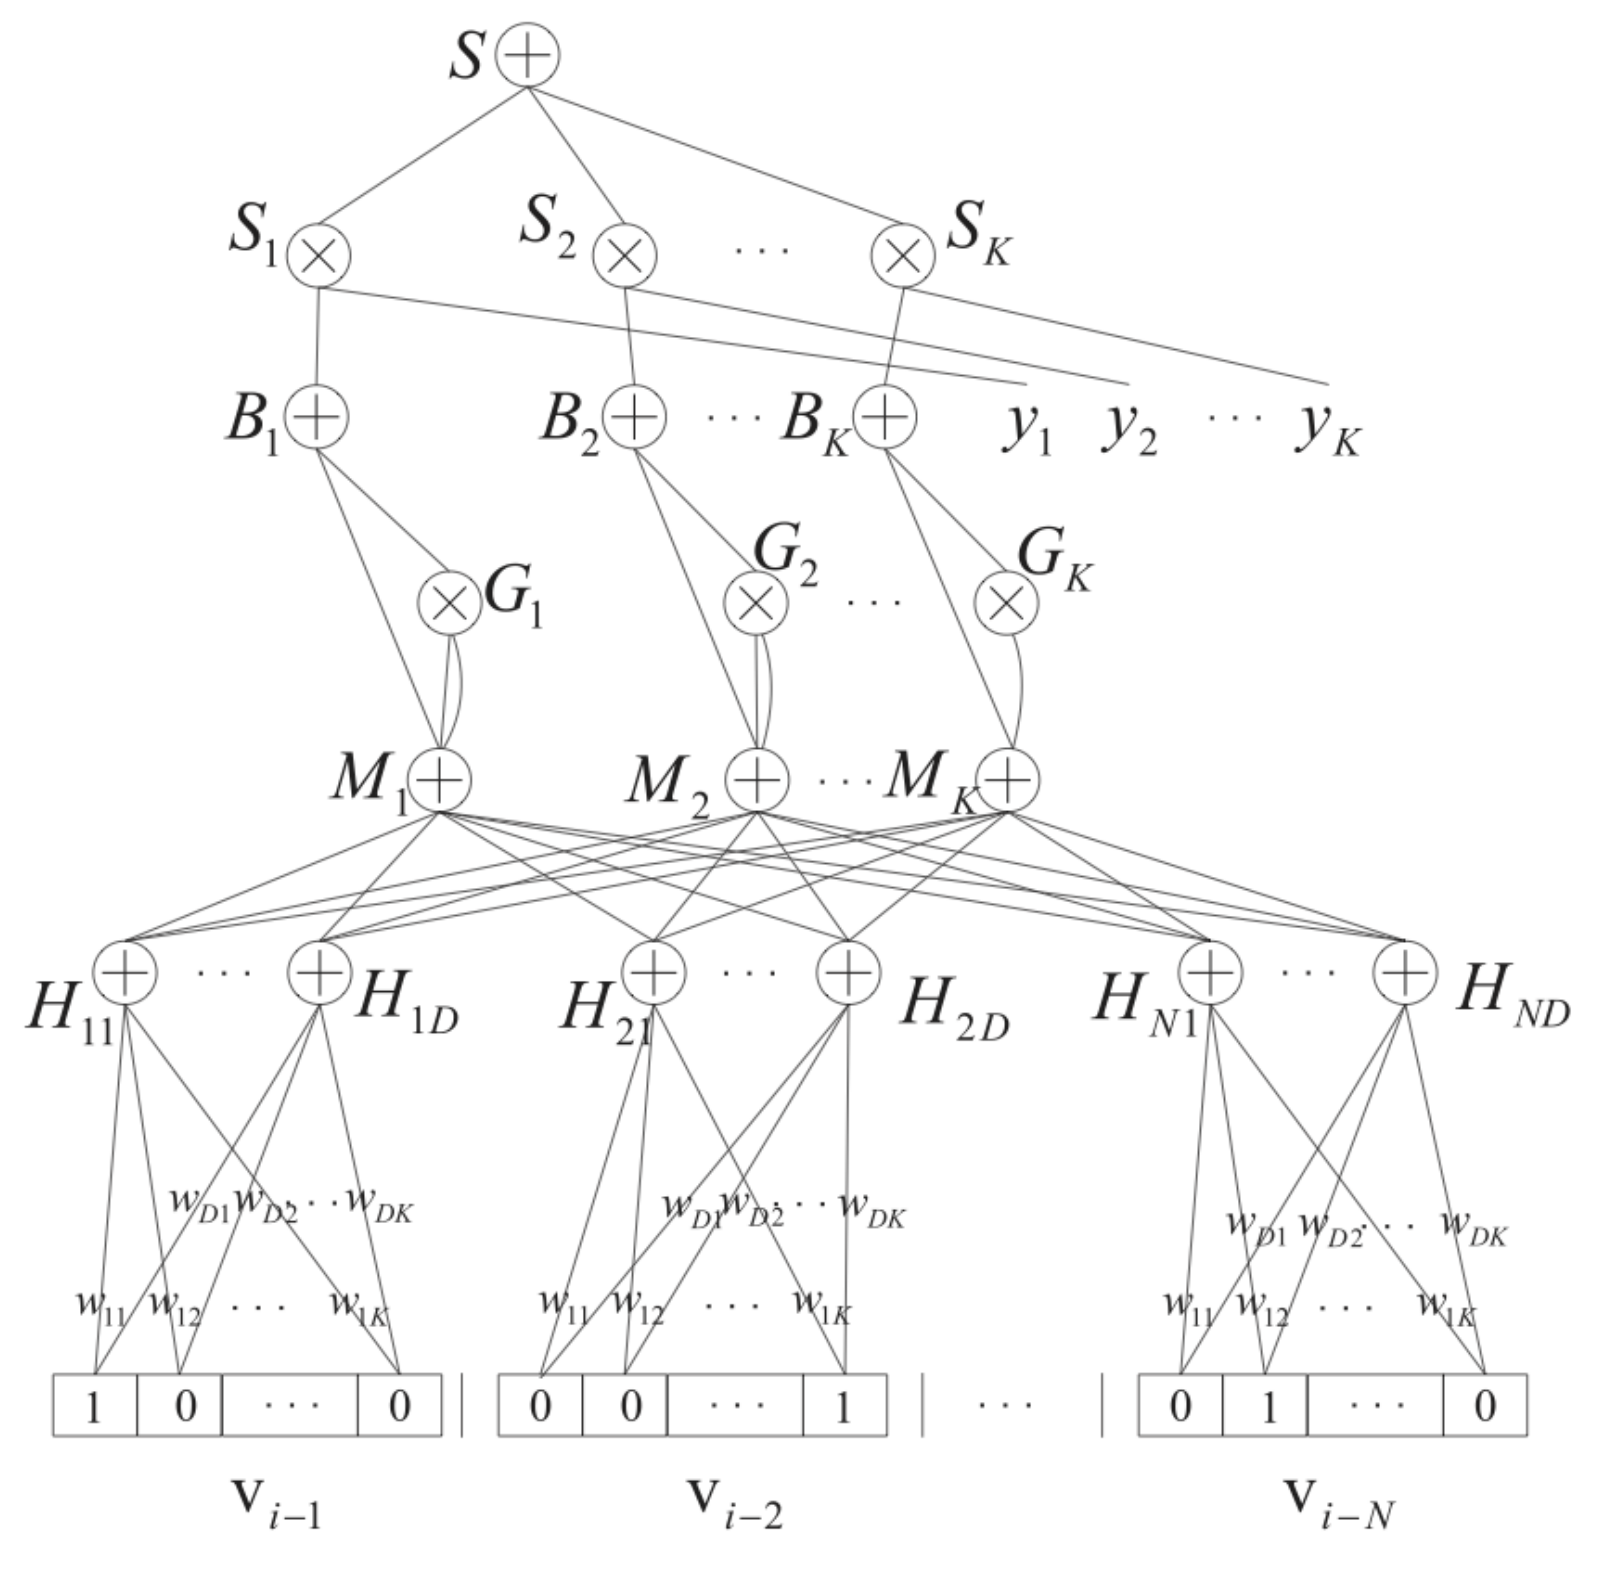
\includegraphics{spn-language.png}}
%        \end{minipage}\begin{minipage}{0.5\textwidth}
%          $\Leftarrow$ Estrutura de SPN construída por Cheng \emph{et al.} (2014) para modelagem de linguagem.
%        \end{minipage}
%      }
%
%      \only<2>{
%        \scalebox{0.7}{
%          \begin{tikzpicture}
%              [scale=.6,auto=left,every node/.style={draw, circle, inner sep = 0pt, minimum width = 0.72cm}]
%            \node (s) at (0,6) {$S$};
%            \node (b1) at (1.5,6) {$B_1$};
%            \node[draw=none] (b) at (3,6) {$\cdots$};
%            \node (bk) at (4.5,6) {$B_K$};
%            \node (m1) at (6,6) {$M_1$};
%            \node[draw=none] (m) at (7.5,6) {$\cdots$};
%            \node (mk) at (9,6) {$M_K$};
%            \node (h11) at (10.5,6) {$H_{11}$};
%            \node[draw=none] (h1) at (12,6) {$\cdots$};
%            \node (h1d) at (13.5,6) {$H_{1D}$};
%            \node (h21) at (15,6) {$H_{22}$};
%            \node[draw=none] (h2) at (16.5,6) {$\cdots$};
%            \node (h2d) at (18,6) {$H_{2D}$};
%            \node[draw=none] (h) at (19.5,6) {$\cdots$};
%            \node (hn1) at (21,6) {$H_{N2}$};
%            \node[draw=none] (hn) at (22.5,6) {$\cdots$};
%            \node (hnd) at (24,6) {$H_{ND}$};
%
%            \node (y1) at (0,0) {$y_1$};
%            \node[draw=none] (y) at (1.5,0) {$\cdots$};
%            \node (yk) at (3,0) {$y_K$};
%
%            \node (v11) at (10.5,0) {\scriptsize $v_{i-1}^1$};
%            \node[draw=none] (v1) at (12,0) {$\cdots$};
%            \node (v1d) at (13.5,0) {\scriptsize $v_{i-1}^K$};
%            \node (v21) at (15,0) {\scriptsize $v_{i-2}^1$};
%            \node[draw=none] (v2) at (16.5,0) {$\cdots$};
%            \node (v2d) at (18,0) {\scriptsize $v_{i-2}^K$};
%            \node[draw=none] (v) at (19.5,0) {$\cdots$};
%            \node (vn1) at (21,0) {\scriptsize $v_{i-N}^1$};
%            \node[draw=none] (vn) at (22.5,0) {$\cdots$};
%            \node (vnd) at (24,0) {\scriptsize $v_{i-N}^K$};
%
%            \foreach \from/\to in {s/y1, s/yk}
%              \draw (\from) edge[->, very thin] (\to);
%
%            \foreach \from/\to in {h11/v11, h11/v1d, h1d/v11, h1d/v1d, h21/v21, h21/v2d, h2d/v21, h2d/v2d, hn1/vn1, hn1/vnd, hnd/vn1, hnd/vnd}
%              \draw (\from) edge[->, very thin] (\to);
%
%            \foreach \from/\to in {s/v11, s/v1d, s/v21, s/v2d, s/vn1, s/vnd}
%              \draw[draw=Blue] (\from) edge[->, very thin] (\to);
%
%            \foreach \from/\to in {b1/v11, b1/v1d, b1/v21, b1/v2d, b1/vn1, b1/vnd}
%              \draw[draw=Red] (\from) edge[->, very thin] (\to);
%            \foreach \from/\to in {bk/v11, bk/v1d, bk/v21, bk/v2d, bk/vn1, bk/vnd}
%              \draw[draw=Red] (\from) edge[->, very thin] (\to);
%
%            \foreach \from/\to in {m1/v11, m1/v1d, m1/v21, m1/v2d, m1/vn1, m1/vnd}
%              \draw[draw=Green] (\from) edge[->, very thin] (\to);
%            \foreach \from/\to in {mk/v11, mk/v1d, mk/v21, mk/v2d, mk/vn1, mk/vnd}
%              \draw[draw=Green] (\from) edge[->, very thin] (\to);
%          \end{tikzpicture}
%        }
%
%        \vspace{1.5em}
%
%        Estrutura da rede bayesiana construída pelo algoritmo de Zhao \emph{et al.} (2015) para representar as mesmas distribuições da SPN para modelagem de linguagem apresentada no slide anterior.
%      }
%    \end{center}
%  \end{frame}

  \begin{frame}
    \frametitle{Conclusões de Zhao \emph{et al.} (2015)}

    \begin{enumerate}
      %\item SPNs não são \textbf{mais poderosas} que BNs com ADDs.
      \item A BN resultante da conversão tem estrutura simples (bipartida), mas é possível relacionar a profundidade de uma SPN com a \emph{treewidth} da BN --- \textbf{mais camadas $\rightarrow$ maior treewidth, distribuições mais complexas}.
      \item Pode haver \textbf{outras técnicas} para converter uma SPN numa BN com uma representação mais compacta e um \emph{treewidth} menor.
      \item Algoritmos para aprender estrutura e parâmetros de SPNs \textbf{podem ser usados} para aprender BNs com ADDs.
    \end{enumerate}
  \end{frame}

  \section{Conclusão}

  \subsection{Distribuições, tratabilidade e compactibilidade}

  \begin{frame}
    \frametitle{Distribuições, tratabilidade e compactibilidade\footnote{\scriptsize POUPART, P. Guest Lecture in STAT946: Deep Learning, University of Waterloo. Disponível em \url{https://www.youtube.com/watch?v=Nm0jNqOnQ2o}}}

    % XXX: compacto = espaço polinomial no número de variáveis
    % XXX: tratável = tempo de inferência é polinomial no número de variáveis

    \scalebox{0.65}{
      \begin{tikzpicture}
        \draw[very thick,draw=Red] (0,0) ellipse (2cm and 1cm);
        \draw[very thick,draw=Blue] (1cm,0) ellipse (5cm and 2cm);
        \draw[very thick,draw=Green] (2cm,0) ellipse (8cm and 3cm);

        \node[text=Red] at (0,0) {\Large $A$};
        \node[text=Blue] at (3.5cm,0) {\Large $B$};
        \node[text=Green] at (8cm,0) {\Large $C$};
      \end{tikzpicture}
    }

    \vspace{1em}

    {\scriptsize \color{Red} $A$: SPNs tratáveis = SPNs compactas = BNs tratáveis}

    {\scriptsize \color{Blue} $B$: BNs compactas}

    {\scriptsize \color{Green} $C$: SPNs gerais = BNs gerais}
  \end{frame}

  \subsection{Considerações finais}

  \begin{frame}
    \frametitle{Considerações finais}

    \begin{itemize}
      \item Redes soma-produto são um \textbf{modelo relativamente novo e promissor}. Estudar sua teoria é interessante porque há muitas questões em aberto e alguns equívocos na literatura, como mostra Peharz (2015)\footnote{PEHARZ, R. Foundations of Sum-Product Networks for Probabilistic Modeling (2015). PhD Thesis.}.
      \item Pretende-se disponibilizar o \textbf{código implementado} (em Go) publicamente na Internet.
    \end{itemize}
  \end{frame}

  \begin{frame}
    \frametitle{Fim}

    Se alguém tiver interesse na apresentação ou na monografia:\\
    {\tt <madeira@ime.usp.br>}

    \vspace{1em}

    \textbf{Perguntas e comentários?}
  \end{frame}
\end{document}
